\chapter{Ingénierie Dirigée par les Modèles}
\label{ch:EA}
 

\section{Genèse et objectifs}

L'Ingénierie Dirigée par les Modèles (IDM) est née du constat que le paradigme 
du « tout est objet », prôné dans les années 1980, a atteint ses limites avec ce 
début de siècle \cite{greenfield2004software}. En effet, face à la croissance de 
la complexité des systèmes logiciels, au coût de la main d'œuvre et de 
maintenance, une approche centrée sur le code, jugé alors seul représentant 
fiable du système, suscitait de moins en moins l'adhésion des industriels et du 
milieu académique. 

Partant de ce constat, l'Object Management Group (OMG) a proposé en novembre 
2000, l'approche MDA (Model Driven Architecture) qui s'inscrit dans le cadre 
plus général de l'IDM et se réalise autour d'un certain nombre de standards tels 
qu'UML, MOF, XML, QVT, etc. Le monde de la recherche s'y est aussitôt intéressé 
pour dégager les principes fondamentaux de l'IDM 
\cite{bezivin2001towards}\cite{kent2002model} \cite{de2002using} et déjouer le 
piège des définitions parfois trop floues qui prêtent à confusion entre les 
concepts liés aux paradigmes d'objet et de modèle \cite{bezivin2004search}. Par 
ailleurs, des industriels comme IBM \cite{booch2004mda} et Microsoft 
\cite{greenfield2004software} ont aussi rendu publiques leur vision de l'IDM. 
Ainsi, l'IDM prend son origine dans la convergence de toutes ces visions et des 
avancées techniques de chacun.

L'originalité de l'IDM ne réside pas dans le recours systématique aux modèles 
dans le développement logiciel comme le laisserait entendre sa terminologie  
\cite{bezivin2004rapport}. Plusieurs méthodes de modélisation telles que Merise 
ou SSADM préconisent aussi l'utilisation de modèles dont le rôle s'achève aux 
phases amont du développement logiciel : l'analyse et la conception. Les modèles 
servent alors à faciliter la communication et compréhension entre les différents 
acteurs mais n'interviennent pas dans la phase de production, de maintien et 
d'évolution. Nous parlons dans ce cas de modèles « contemplatifs ». 

L'IDM a pour objectif de rendre les modèles « productifs » sur tout le cycle de 
vie du système et à tout niveau d'abstraction. Pour y parvenir, les modèles 
doivent être décrits formellement pour être interprétés et exécutés par une 
machine. Dès lors, ces modèles permettent d'industrialiser la production 
logicielle, jusque-là centrée sur le code produit par l'informaticien 
\cite{bezivin2005unification}.

En mettant à profit des disciplines comme la modélisation par objets, 
l'ingénierie des langages, la compilation de langages, les méthodes formelles, 
la programmation par composants, etc., l'IDM offre un cadre intégrateur reposant 
sur quelques concepts fondamentaux : la notion de modèle et la relation 
\textit{ReprésentationDe}, la notion de métamodèle et la relation 
\textit{ConformeÀ}.

\section{Concepts fondamentaux}
\subsection{Modèle et ReprésentationDe}
La notion de modèle est centrale dans l'IDM car, comme nous venons de voir, 
l'enjeu de cette approche est de rendre les modèles productifs sur tout le cycle 
de vie du système. Il n'existe pas de définition universelle de la notion de 
modèle. En nous appuyant sur les définitions données dans les travaux 
\cite{minsky1967computation} \cite{bezivin2001towards} et 
\cite{seidewitz2003models}, nous adoptons la définition suivante du terme modèle 
:

\begin{definition}
Un modèle est une abstraction d'un système, selon le bon point de vue, qui 
permet de répondre à des questions prédéfinies sur ce système en lieu et place 
de celui-ci.
\end{definition}

De cette définition découle la première relation fondamentale de l'IDM qui lie 
le modèle et le système qu'il représente. Celle-ci est nommée 
\textit{Représente} et notée $(\mu)$. Bien que la relation 
\textit{Représente} ne soit pas nouvelle dans l'ingénierie logicielle 
(Merise, UML), l'IDM a permis d'en définir les contours \cite{atkinson2003model} 
\cite{seidewitz2003models} \cite{bezivin2004search}.

\begin{figure}[!htbp]
 \begin{center}
  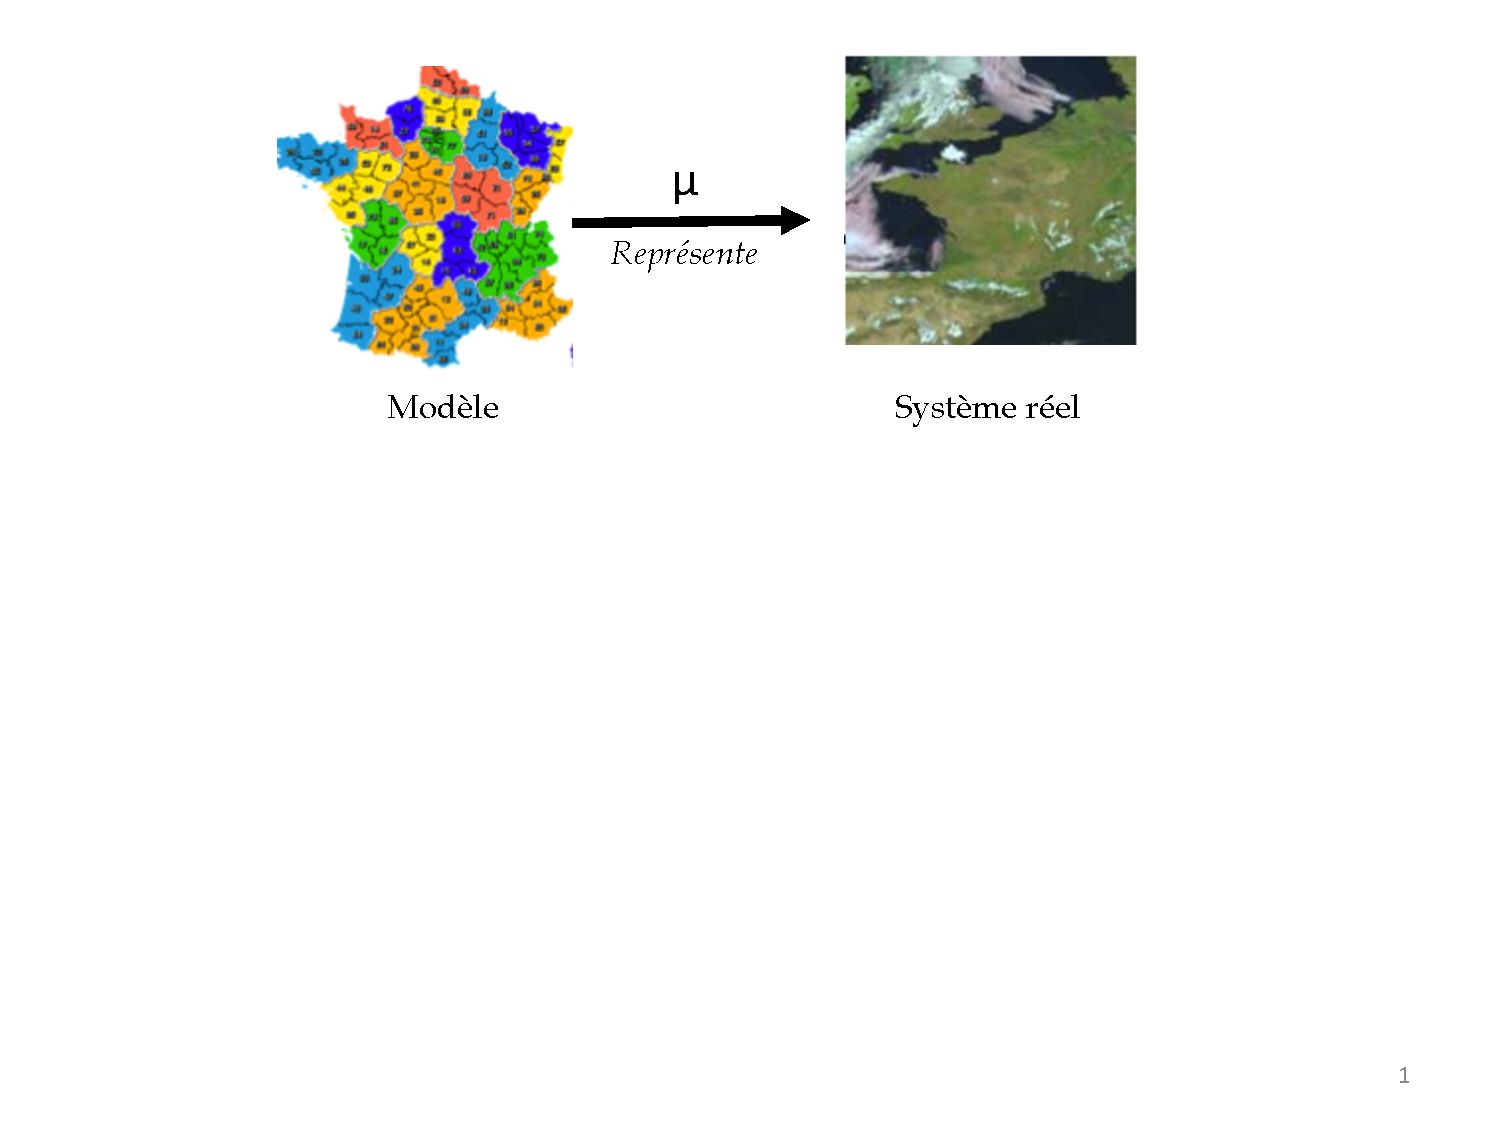
\includegraphics[trim= 0cm 12cm 0cm 0cm, width=1\textwidth]{figures/images/Chapitre1/favresystememodele.pdf}
 \end{center}
 \caption{Relation entre système et modèle \protect\cite{favre2006ingenierie}}
 \label{fig:systemModele}
\end{figure}

Cette définition n'est pas restreinte à l'informatique et pourrait s'appliquer à 
n'importe quel système. 
La figure~\ref{fig:systemModele} reprend l'exemple connu de la cartographie où 
une carte géographique joue le rôle de modèle pour une région donnée jouant 
alors le rôle de système modélisé. 

L'intérêt de l'IDM est de produire des modèles exploitables informatiquement. 
Ceci n'est possible que si ces modèles sont décrits par des langages formels. Il 
devient alors important de bien définir ces langages à l'aide de métamodèles

\subsection{Métamodèle et ConformeÀ}
L'originalité de l'IDM ne réside pas dans la relation ReprésentationDe qui 
trouve plutôt son origine dans les méthodes de modélisation telles que Merise ou 
SSADM. L'apport de l'IDM est dans l'utilisation systématique de métamodèles pour 
la description des langages de modélisation. 

Il existe plusieurs définitions de la notion de métamodèle dans la littérature. 
Cependant la définition suivante est communément admise 
\cite{bezivin2004rapport}.

\begin{definition}
Un métamodèle est un modèle du langage de modélisation qui sert à exprimer les 
modèles.
\end{definition}
Une autre définition courante mais erronée de la notion de métamodèle suppose 
qu'un métamodèle est un modèle d'un modèle. La figure~\ref{fig:modelofmodel} 
reprend l'exemple de la cartographie évoquée plus haut. Nous appliquons 
récursivement la relation \textit{ReprésentationDe} $(\mu)$ au territoire 
français. Ici une carte de la France joue le rôle de modèle du territoire 
français et un fichier XML joue le rôle de modèle de la carte. Dans ce contre 
exemple, le fichier XML n'est pas un métamodèle de la France. Un métamodèle 
n'est donc pas un modèle d'un modèle.

\begin{figure}[!htbp]
 \begin{center}
  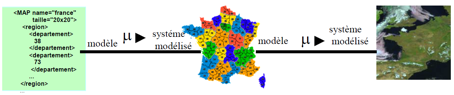
\includegraphics[width=1\textwidth]{figures/images/Chapitre1/modelofmodel.png}
 \end{center}
 \caption{Modèle de modèle selon l'exemple de la cartographie 
\protect\cite{favre2006ingenierie}}
 \label{fig:modelofmodel}
\end{figure}

Par ailleurs, le concept de métamodèle induit la deuxième relation fondamentale 
de l'IDM liant un modèle à son métamodèle. Cette relation est nommée 
\textit{ConformeÀ} et notée $\chi$ \cite{bezivin2004search} 
\cite{favre2004towards}. La figure \ref{fig:carteFavre} reprend l'exemple de la 
cartographie où la légende de la carte joue le rôle de métamodèle ($\chi$) pour 
une carte de la France. En effet, pour être lisible, la carte doit être conforme 
à la légende.

\begin{figure}[!htbp]
 \begin{center}
  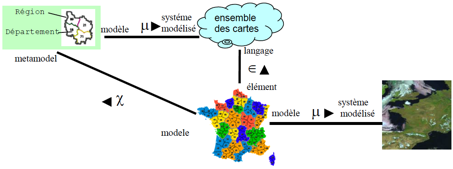
\includegraphics[width=1\textwidth]{figures/images/Chapitre1/cartecompleteIDM.png}
 \end{center}
 \caption{Relations entre système, modèles, métamodèle et langage de 
modélisation \protect\cite{favre2006ingenierie}}
 \label{fig:carteFavre}
\end{figure}

\section{Transformation de modèle}
Dans la partie précédente, nous avons introduit les concepts fondamentaux de 
l'IDM que représentent la notion de modèle et la relation 
\textit{ReprésentationDe} ainsi que la notion de métamodèle et la relation 
\textit{ConformeÀ}. Comme expliqué, la préoccupation majeure de l'IDM est de 
rendre les modèles opérationnels sur tout le cycle de vie des systèmes 
logiciels, depuis l'analyse et la conception jusqu'à la maintenance et 
l'évolution. Ainsi, la transformation de modèle se retrouve au cœur de l'IDM car 
c'est à travers elle que se fait l'automatisation des traitements apportés aux 
modèles. Nous allons d'abord donner une définition de la notion de 
transformation de modèle puis en présenter les types et les usages.

\subsection{Définition de la transformation de modèle}
L'OMG définit une transformation de modèle comme «~le processus consistant à 
convertir un modèle en un autre modèle d'un même système~» \cite{omg2011meta}. 

\cite{kleppe2003mda} proposent une définition moins générique en insistant sur 
l'aspect automatique de ce processus, ainsi, «~une transformation de modèle 
consiste en la génération automatique d'un modèle source en un modèle cible, 
selon une description établie de cette transformation~». Cette définition 
implique aussi qu'une transformation est décrite à un plus haut niveau 
d'abstraction : au niveau d'un métamodèle auquel elle doit se conformer. 

\cite{mens2006taxonomy} étendent cette définition en considérant qu'une 
transformation est une opération qui peut avoir en entrée un ou plusieurs 
modèles source et en sortie un ou plusieurs modèles cible~: 

\begin{definition}
Une transformation génère automatiquement un ou plusieurs modèles cible à partir 
d'un ou plusieurs modèles source, selon une description établie de la 
transformation. 
\end{definition}

C'est cette dernière définition que nous allons adopter dans ce document. Par 
ailleurs, notons que, si les métamodèles source et cible sont différents, la 
transformation est dite exogène. Si les métamodèles source et cible 
correspondent au même métamodèle, la transformation est dite endogène. Ces 
termes ont été introduits par \cite{mens2006taxonomy}.

\subsection{Composants d'une transformation de modèle} 
La figure \ref{fig:composantTransfo} illustre les composants d'une 
transformation de modèle~:~les modèles source, les modèles cible, la définition 
de la transformation et le moteur qui va opérer la transformation selon sa 
définition. 

La description de la transformation spécifie comment un ou plusieurs modèles 
source sont transformés en un ou plusieurs modèles cible. Elle est écrite dans 
un langage de transformation de modèle. Par exemple, si c'est un langage à base 
de règles, la description de la transformation consiste en un ensemble de règles 
de transformation à opérer \cite{kleppe2003mda}. 

Un moteur de transformation exécute ou interprète la description. Il applique 
donc la description aux modèles source pour produire les modèles cible en 
suivant les étapes ci-dessous \cite{tratt2005model}~:

\begin{itemize}
\item Identifier l'élément du ou des modèles source à transformer.
\item Pour chaque élément identifié, produire l'élément cible qui lui est 
associé dans le ou les modèles cible.
\item Produire une trace de la transformation qui lie les éléments du ou des 
modèles cibles aux éléments du ou des modèles source.
\end{itemize}

\begin{figure}[!htbp]
 \begin{center}
   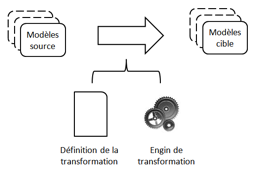
\includegraphics[width=0.7\textwidth]{figures/images/Chapitre1/composanttransfo.png}
 \end{center}
 \caption{Composants d'une transformation de modèle}
 \label{fig:composantTransfo}
\end{figure}

\subsection{Usages de la transformation de modèles }
Les transformations de modèles sont au cœur d'une démarche dirigée par les 
modèles~:~elles permettent d'automatiser les manipulations subies par les 
modèles telles que la modification, la création, l'adaptation, la composition ou 
encore le filtrage de modèles, à travers la réutilisation systématique 
d'informations contenues dans les modèles existants. 

Il est possible de recourir aux transformations de modèles sur tout le cycle de 
vie d'un système. Les usages les plus répondus sont le raffinement, 
l'intégration d'outils, la composition, l'analyse, la simulation et 
l'optimisation que nous présentons dans la suite de ce document. 

\begin{description}

\item \textbf{Raffinement}

Le raffinement consiste à rajouter plus de détails au modèle initial. Ce type de 
transformation peut aussi bien être endogène (métamodèles source et cible 
identique) ou exogène (métamodèle source et cible différents). Le raffinement se 
prête parfaitement à toute la partie descendante du cycle en V où les modèles 
passent à des niveaux d'abstraction plus bas. Ceci revient à faire des 
transformations successives de type modèle-à-modèle et une transformation de 
type modèle-à-texte pour aboutir au code final.

Raffiner un modèle revient à décomposer des concepts de haut niveau, à choisir 
un algorithme particulier, à spécialiser un concept pour un contexte donné ou 
encore à le concrétiser sous forme d'une solution exécutable par une machine en 
générant le code à partir de modèles de plus haut niveau d'abstraction 
\cite{czarnecki2000intentional}. 

\item \textbf{Intégration d'outil}

Il existe une panoplie d'outils disponibles pour créer, manipuler, analyser ou 
encore simuler des modèles. Souvent ces outils utilisent des métamodèles 
internes et des espaces techniques qui leurs sont propres. Ainsi, l'échange de 
modèle entre ces outils est compromis et l'interopérabilité est fortement 
entravée. L'utilisateur se trouve obligé d'utiliser un seul et même outil sur 
tout le cycle de vie du système et ne peut donc pas tirer avantage des 
possibilités offertes par d'autres outils plus adaptés à ses besoins à certaines 
étapes.

L'intégration d'outil est une solution pour palier la divergence syntaxique et 
sémantique des outils et des langages de modélisation par le biais la 
transformation de modèle \cite{tratt2005model}. Ce type de transformation permet 
de naviguer entre deux métamodèles, de synchroniser des modèles qui évoluent 
séparément sur des outils distincts, de faire des mapping entre métamodèles pour 
maintenir la cohérence des modèles conformes à ces métamodèles. Il sera donc 
possible de faire appel à des outils mieux adaptés à chaque étape du cycle de 
vie.

\item \textbf{Composition}

Pour réduire la complexité inhérente à la modélisation et à l'analyse de grands 
systèmes, tels que les Smart Grids par exemple, il est possible d'adopter une 
approche par points de vue qui permet de séparer les préoccupations. Les modèles 
produits correspondent donc à ces différents points de vue qu'on peut ainsi 
valider séparément dans un premier temps. A l'issue de cette approche modulaire, 
on pourra composer ces modèles, c'est-à-dire les assembler, pour aboutir un 
modèle global du système.

Dans le cas le plus simple, les deux modèles à composer sont conformes à un même 
métamodèle. Cependant, il est aussi possible de composer deux modèles conformes 
à deux métamodèles différents. 

Les deux modèles à composer peuvent aussi présenter des concepts en commun. Deux 
techniques existent pour composer des modèles, que nous illustrons dans la 
figure \ref{fig:compoExemple}~:

\begin{itemize}
\item La première technique consiste à les fusionner. Dans ce cas, le modèle 
final résultant de la composition doit contenir toutes les informations issues 
des modèles initiaux, sans duplication des informations communes 
\cite{bezivin2006canonical}.
\cite{fleurey2008generic} présente un framework générique capable de composer 
des modèles indépendamment de leurs langages de modélisation. L'approche 
consiste à identifier les éléments qui représentent le même concept dans les 
deux modèles à composer et à les fusionner dans un nouveau modèle qui représente 
une vue intégrée de ces concepts. Il est aussi possible de spécialiser le 
framework pour un métamodèle particulier mais qui reste conforme au MOF.

\item La deuxième technique consiste à les tisser. Dans ce cas, on crée des 
correspondances entre les éléments qui représentent un même concept. Un 
métamodèle générique est créé pour définir les correspondances qui sont donc 
modélisées dans le modèle final. On y retrouve donc les éléments en commun 
dupliqués mais liés par un lien de correspondance. 
\end{itemize}

Il est à noter que le modèle issu du tissage de deux modèles $M_{A}$ et $M_{B}$ 
peut être utilisé comme modèle intermédiaire que l'on note $M_{T}$ pour la 
fusion de $M_{A}$ et $M_{B}$. Dans ce cas L'opération de fusion consiste à 
produire un modèle $M_{AB}$ en prenant comme entrée $M_{A}$, $M_{B}$ et $M_{T}$. 
Cette technique est notamment utilisée par \cite{del2007semi} pour la 
composition semi-automatique de modèles.

\begin{figure}[!htbp]
 \begin{center}
  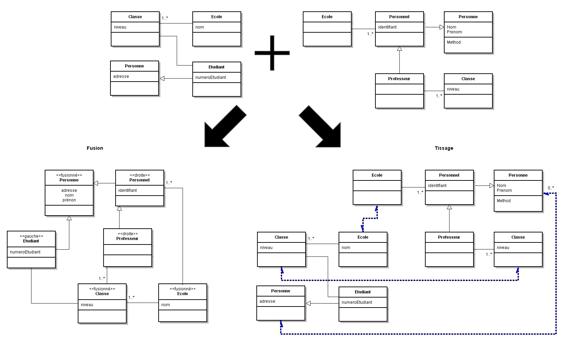
\includegraphics[width=1\textwidth]{figures/images/Chapitre1/compoExemple.png}
 \end{center}
 \caption{Exemple de composition de deux modèles}
 \label{fig:compoExemple}
\end{figure}

\item \textbf{Simulation}

La transformation de modèle peut être utilisée pour simuler des modèles. En 
effet, une transformation de modèle peut mettre à jour le système modélisé. Dans 
ce cas, le modèle cible est une mise à jour du modèle source et la 
transformation est de type sur-place (modèles source et cible confondus). 

Par exemple, \cite{syriani2011multi} simule un comportement simple d'un jeu de 
Pacman en utilisant la transformation de modèle. La transformation spécifie les 
règles de transition qu'une instance du jeu peut prendre (Pacman et fantôme se 
trouvant dans la même case, Pacman et pomme se trouvant dans la même case, 
etc.). En ingénierie des langages, ceci revient à définir la sémantique 
opérationnelle d'un langage de modélisation. L'exécution de la transformation 
anime le modèle en fonction du comportement qu'on lui confère.

La transformation peut aussi être utilisée comme intermédiaire dans la 
simulation de modèle. Des modèles en entrée d'un outil de simulation externe 
sont produits par une transformation des modèles qu'on souhaite simuler. Cette 
technique permet de tirer profit d'outils de simulation existant sur le marché 
en utilisant l'intégration d'outils.

\item \textbf{Analyse et optimisation}

La transformation de modèle peut être utilisée pour les activités d'analyse de 
modèle. Une analyse simple telle que le calcul de métrique de similarité entre 
deux modèles via la transformation de modèle est donnée dans \cite{del2007semi} 
avec un modèle de transformation écrit en ATL \cite{jouault2006transforming}. 

Des analyses plus complexes sont possibles grâce à l'intégration d'outils 
d'analyse externes vers lesquels les modèles source sont transformés.

\cite{biehl2010integrating} propose d'utiliser la transformation de modèle pour 
l'analyse de sûreté de fonctionnement dans le domaine de l'automobile. Les 
modèles source sont transformés en modèles conformes au métamodèle de l'outil 
d'analyse de sûreté de fonctionnement retenu.
 
L'optimisation vise à améliorer les propriétés non fonctionnelles des modèles 
telle que l'évolutivité, la fiabilité, la modularité, etc. L'optimisation est 
typiquement utilisée sur les modèles d'architecture. Les transformations 
utilisées pour l'optimisation sont de types endogènes car on cherche à affiner 
la conception de modèles existants. La réingénierie est un exemple de 
transformation utilisée pour optimiser les modèles~:~on cherche à améliorer la 
maintenabilité, la lisibilité et l'évolutivité des modèles.

\end{description}

\subsection{Approches existantes pour la transformation de modèle}  
Le recours à la transformation de modèle est l'objet de recherches informatiques 
antérieures à l'apparition de l'approche IDM. Par exemple, les compilateurs 
utilisent la transformation pour passer du code source au fichier binaire 
\cite{aho1985compilers}. Ce type de transformation est restreint au domaine de 
la programmation informatique. La transformation de modèle embrasse un domaine 
plus large encore.

Nous trouvons dans la littérature plus d'une trentaine d'approches différentes 
de transformation de modèle \cite{syriani2011multi}. Czarnecki et Helsen 
proposent une classification de ces approches selon plusieurs critères tels que 
le paradigme retenu pour définir la transformation, la relation entre les 
modèles sources et cibles, la directivité de la transformation, le nombre de 
modèles cible et source, l'orchestration et l'ordonnancement des règles de 
transformation, etc. \cite{czarnecki2006feature}.

\cite{blanc2011mda} retient trois grandes catégories d'approches~:

\begin{itemize}
\item Par programmation

Les modèles offrent une interface qui permet d'écrire les transformations dans 
un langage de programmation. Mais cette technique relève plus de la 
programmation que de la modélisation. Ce sont en fait des applications 
informatiques qui ont la particularité de manipuler des modèles. L'avantage de 
cette approche est que l'on utilise un langage de programmation généraliste tel 
que Java ou C++ pour écrire les transformations. Ainsi le programmeur n'a pas 
besoin d'apprendre un nouveau langage. Cependant ces applications ont tendance à 
devenir difficilement maintenables. 

\item Par template 

Dans cette approche on définit des canevas des modèles cibles. Ces modèles 
contiennent des paramètres qui seront remplacés par les informations contenues 
dans les modèles source. Ce type de transformation est souvent utilisé pour les 
transformations modèle-à-texte et est associé au visitor-pattern qui va 
traverser la structure interne du modèle source. Cette approche est utilisée par 
l'outil Enterprise Architect par exemple. 

\item Par modélisation

Cette approche vise à appliquer les principes de l'IDM aux transformations de 
modèles elles-mêmes. Ainsi, on produit des modèles de transformation prennes, 
réutilisables et indépendants des plates-formes d'exécution 
\cite{bezivin2006model}. 

Pour cela, on utilise des langages de modélisation dédiés à l'activité de 
transformation de modèles. Cette approche considère donc la transformation comme 
un modèle à part entière conforme à un métamodèle de transformation. La figure 
\ref{fig:TransfoPrincipe} , illustre cette approche en positionnant la 
transformation sur les différents niveaux d'abstraction de l'IDM. Elle corrobore 
ainsi la vision unificatrice de l'IDM à travers le paradigme du « tout est 
modèle » \cite{bezivin2005unification}. Le langage de transformation ATL, que 
nous présentons dans la section~\ref{sec:ATL}, a été développé dans ce sens. 

\end{itemize}

\begin{figure}[!htbp]
 \begin{center}
  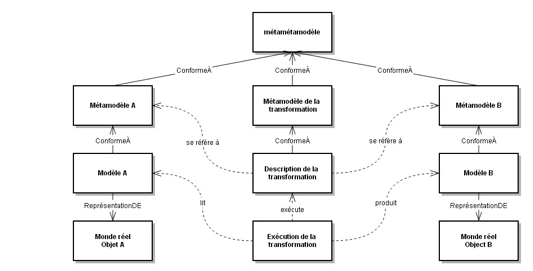
\includegraphics[width=1\textwidth]{figures/images/Chapitre1/transfoPrincipe.png}
 \end{center}
 \caption{Méta niveaux d'une transformation de modèle}
 \label{fig:TransfoPrincipe}
\end{figure}

\section{Langages et outils pour la transformation de modèle}
Dans cette section, nous introduisons succinctement quelques langages et outils 
dédiés à la transformation de modèles, sans viser à l'exhaustivité.

\subsection{ATL}
\label{sec:ATL}
Atlas Transformation Language (ATL) \cite{jouault2006transforming} 
\cite{jouault2008atl} est né de la volonté de proposer des langages de 
modélisation dédiés à la transformation de modèle en définissant un métamodèle 
et des outils pour l'exécution des transformations. Il permet de réaliser des 
transformations de type modèle-à-modèle et de type modèle-à-texte.

ATL  est un langage hybride (déclaratif et impératif) à base de règles OCL (OMG 
2014). Une règle déclarative, appelée Matched rule, permet de décrire 
l'implémentation de mapping simples entre les modèles source et cible en 
utilisant des patrons source (\textit{InPattern}) mappés avec les éléments 
source et des patrons cibles (\textit{outPattern}) mappés avec les éléments 
cible. 

L'approche impérative explicite les étapes d'exécution de la transformation à 
travers les Helpers. Ce mécanisme de Helpers permet en outre d'éviter la 
redondance de code et la création de longues règles écrites en OCL, ce qui 
confère une meilleure lisibilité aux programmes ATL. 

Une transformation écrite en ATL est composée d'un ensemble de règles qui 
spécifient comment créer et initialiser les éléments des modèles cible. Il n'est 
pas possible de spécifier l'ordre d'exécution des règles de transformation. Cet 
ordre est établi automatiquement, exception faite pour les \textit{lazy rules} 
qui ont besoin qu'on fasse spécifiquement appel à elles. ATL est conforme au 
méta-métamodèle MOF et est doté d'une syntaxe concrète textuelle. Il est intégré 
à l'environnement Eclipse. Une transformation prend en entrée un ensemble de 
modèles conformes à Ecore (EMF 2014) ou KM3 \cite{jouault2006km3}.

ATL ne prend pas en charge les transformations incrémentales. Il commence par 
lire entièrement les modèles source et génère des modèles cible complet. Les 
modifications manuelles dans les modèles cible ne sont donc pas préservées si 
l'on opère une nouvelle transformation.

ATL peut réaliser des transformations sur  place, c'est-à-dire, une 
transformation où le modèle source et le modèle source sont confondus en 
utilisant le mode raffinement de modèle. Cependant ce mode présente quelques 
limitations avec certaines fonctionnalités comme celle des \textit{lazy rules}.

\subsection{QVT}
Le framework Query View Transformation (QVT) \cite{kurtev2008state} 
\cite{omg2011meta} a rejoint la batterie de standards de l'OMG. Le métamodèle de 
QVT est conforme au MOF. Comme ATL, QVT se base sur OCL pour accéder aux 
éléments des modèles.
QVT définit trois langages de transformation de type modèle-à-modèle. 
QVT-Relations (QVT-R) et QVT-Core (QVT-C) sont des langages déclaratifs qui 
adressent deux niveaux d'abstraction différents. QVT-Operational Mappings 
(QVT-OM) est un langage impératif qui étend QVT-R et QVT-C.

QVT-R est un langage de transformation de haut niveau d'abstraction doté de 
syntaxes concrètes textuelle et graphique. Les transformations, 
bidirectionnelles, sont spécifiées sous forme de relations entre les modèles 
source et cible. Une transformation a pour but de vérifier la cohérence entre 
deux modèles, renforcer la cohérence en modifiant le modèle cible, synchroniser 
deux modèles ou encore pour raffiner un modèle par une transformation sur-place. 
La sémantique de QVT-R est définie par une transformation vers QVT-C.

QVT-C est un langage de transformation de bas niveau qui sert de base pour 
QVT-R. Les deux ont le même niveau d'expressivité. Une transformation consiste 
en la déclaration de mapping entre les métamodèles source et cible en utilisant 
des patterns. Contrairement à QVT-R, la traçabilité est explicitement définie à 
travers les liens entre les métamodèles.

QVT-OM est un langage de transformation impératif qui étend QVT-R avec des 
constructions impératives basée sur une extension impérative de OCL. Les 
transformations sont unidirectionnelles mais établissent explicitement des 
modèles de traçabilité.

QVT est aussi doté d'un mécanisme de \textit{graybox} qui permet de faire appel 
à des algorithmes complexes écrits dans n'importe quel langage de programmation 
et d'utiliser des librairies existantes. Mais ce mécanisme rend la 
transformation opaque puisqu'il n'est pas contrôlé par le moteur d'exécution. 
Nous pouvons citer SmartQVT ou encore ModelMorf comme machines d'exécution de 
transformation écrite en QVT.

\subsection{Kermeta}
Kermeta est un langage généraliste de méta-modélisation exécutable et de 
méta-programmation orientée objet qui peut aussi décrire des transformations de 
modèle. Intégré à EMF, il est doté d'un métamodèle conforme au MOF qu'il étend 
avec un langage d'action impératif utilisé pour écrire le corps des opérations 
définies sur les concepts d'une syntaxe abstraite (ce qui revient à doter une 
syntaxe abstraite d'une sémantique opérationnelle). On peut ainsi décrire 
n'importe quel traitement sur un modèle ce qui est assimilé à une transformation 
de modèle.

Le langage d'action de Kermeta permet d'écrire des expressions impératives qui 
spécifient explicitement la construction des éléments des modèles cible. A 
l'inverse de QVT-OM, Kermeta n'est pas un langage à base de règles.  
Kermeta est capable de gérer les exceptions mais les transformations 
multidirectionnelles ne sont pas supportées par les outils d'exécution. Il en 
est de même pour la transformation incrémentale. Les modèles source sont lus en 
une seule fois et les modèles cible sont produits complets lors de l'exécution 
de la transformation.

\subsection{Acceleo}
to be continued

\section{L'Ingénierie Dirigée par les Modèles pour l'Architecture d'Entreprise}

L'IDM se cantonne souvent au processus de développement logiciel en offrant une aide supplémentaire à l'analyse et la validation des modèles de spécification et en automatisant certaines tâches à travers la génération de code par exemple. Mais des disciplines plus orientées métier telle que l'EA peuvent aussi tirer partie des avantages qu'apporte l'IDM à l'ingénierie logicielle. 

\subsection{Méta-modélisation en Architecture d'Entreprise}

Les cadres d'architecture contribuent à réduire considérablement la complexité liée à un système telle que l'entreprise en décomposant celle-ci en plusieurs vues. Les architectes d'entreprise doivent ensuite représenter les artefacts qui composent ces différentes vue. Le recours aux techniques de modélisation n'est donc pas étranger à l'EA. Les architectes d'entreprise ont besoin d'une représentation claire et pertinente des composants de l'entreprise pour leur propre compréhension mais aussi à des fins de communication avec les autres parties prenantes comme les experts métier, les architectes applicatifs ou encore les responsables stratégiques. 

Souvent, les cadres d'architecture ne préconisent pas de langages de modélisation en particulier et se contentent d'ériger un ensemble de bonnes pratiques. Pour représenter l'entreprise, les architectes utilisent alors des notations qui leurs sont propres. Deux architectes appartenant à des filiales différentes d'une même entreprise et utilisant des notations différentes sont susceptibles d'engendrer des problèmes de communication et d'interopérabilité à l'échelle de l'entreprise. 

Graphiques ou textuelles, ces notations manquent cruellement d'une sémantique précise et formalisée. L'apparition de difficultés liées à la compréhension et à la collaboration entre les acteurs impliqués dans l'EA est alors inéluctable. L'architecture de l'entreprise perd alors de sa crédibilité en tant que référentiel d'entreprise. Les outils de visualisation et d'analyse sont d'autant plus difficiles à développer à cause du manque de formalisme des modèles purement contemplatifs.

L'\textit{Open Group} propose de mettre en cohérence les notations utilisés en EA en créant un langage de modélisation standardisé nommé Archimate. Archimate sert ainsi à décrire l'entreprise, sa structure organisationnelle, ses processus, ses règles métier ou encore son SI. Archimate est un langage de représentation graphique utilisé pour documenter et à communier les architectures d'entreprise au sein d'une même organisation ou entre différentes organisations. Archimate est en outre étroitement lié au cadre d'architecture TOGAF. 

Le métamodèle d'Archimate est concis mais vise à couvrir la majorité des concepts intervenants dans la création d'une architecture d'entreprise. Archimate utilise trois vues~:~métier, applicative et technique. Pour chacune des vues, trois types d'éléments différents sont spécifiés~:~structure active, comportement et structure passive. Les structures actives correspondent aux éléments dotés d'un comportement tels qu'un acteur métier, un module applicatif ou encore un élément de l'infrastructure technique. Le comportement correspond à ensemble d'activités ou de tâches poursuivie par un ou plusieurs éléments de la structure active. Il peut s'agit par exemple d'un processus métier. Les structures passives correspondent aux éléments manipulés par le comportement comme par exemple les objets métier. Archimate associe des couleurs différentes aux éléments en fonction de leur type (voir figure \ref{fig:archimate}). Les éléments de type structure active sont bleus, ceux de type comportement sont jaunes et enfin ceux de type structure passive sont verts. 

Le métamodèle du langage Archimate est un adossé d'une syntaxe concrète graphique permettant visualiser les modèles. Mais aucune sémantique standard d'exécution n'est formalisée. Les modèles d'architecture sont ainsi souvent purement contemplatifs et les outils implémentant Archimate n'offrent pas la possibilité d'exécuter ces modèles à des fins d'analyse de structure et de comportement. 

\begin{figure}[!htbp]
 \begin{center}
   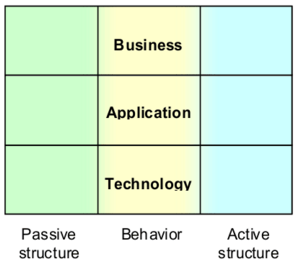
\includegraphics[width=0.5\textwidth]{figures/images/Chapitre1/archimate_core.png}
 \end{center}
 \caption{Composants du langage Archimate}
 \label{fig:archimate}
\end{figure}



\subsection{Approches d'Architecture d'Entreprise recourant à l'Ingénierie Dirigée par les Modèles}

L'IDM a prouvé sa capacité à adresser des systèmes complexes \cite{france2007model}. L'application des techniques de l'IDM aux approches d'EA font l'objet de quelques rares travaux \cite{bruneliere2013support}. Les travaux de Frankel et al. \cite{frankel2003zachman} font figure de précurseurs. Ces derniers décrivent un mapping entre le cadre Zachman et les vues MDA (figure \ref{fig:mapping-zachman-mda}). Mais le périmètre de ces travaux se réduit à l'architecture IT de l'entreprise plutôt qu'à l'entreprise dans son ensemble.

\begin{figure}
 \begin{center}
   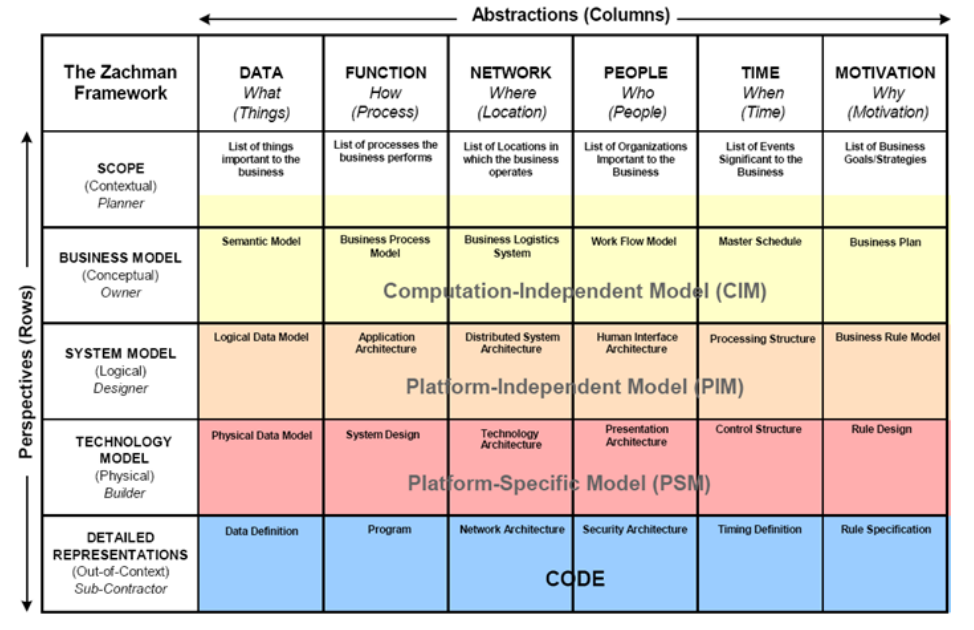
\includegraphics[width=\textwidth]{figures/images/Chapitre1/mapping_zachman_mda.png}
 \end{center}
 \caption{Mapping Zachman/MDA \protect\cite{frankel2003zachman}}
 \label{fig:mapping-zachman-mda}
\end{figure}

Clark et al. \cite{clark_towards_2014} proposent d'étendre la démarche MDA,  traditionnellement appliquée au développement de systèmes informatiques, à l'ensemble de l'entreprise pour mettre en place une organisation dirigée par les modèles ou MDO (\textit{Model Driven Organisation}). Comme l'illustre la figure \ref{fig:mdo}, une MDO comprend un modèle de l'organisation (\textit{Model of the Organization}), d'un modèle spécifique à une plateforme (\textit{Platform Specific Model}) et d'une plateforme d'organisation (\textit{Platform for Organization}). 

\begin{figure}[!htbp]
 \begin{center}
   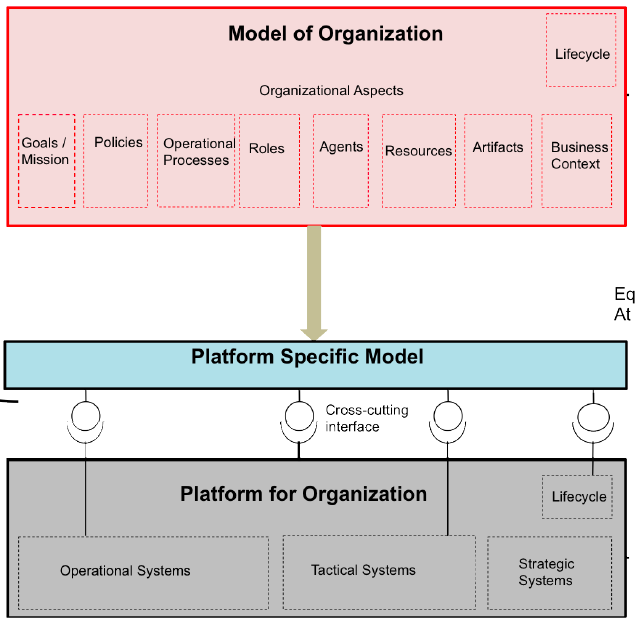
\includegraphics[width=0.7\textwidth]{figures/images/Chapitre1/mdo.png}
 \end{center}
 \caption{Architecture d'une organisation dirigée par les modèles (à remplacer par une belle figure) \protect\cite{clark_towards_2014}}
 \label{fig:mdo}
\end{figure}

Le modèle de l'organisation correspond à l'ensemble des modèles métier (processus, objectifs, acteurs, ressources, etc.). Pour réaliser ses processus métier, une organisation a besoin des technologies de l'information. L'ensemble du système informatique correspond alors à la plateforme opérationnelle de l'entreprise. Comme pour MDA, le modèle spécifique à une plateforme est dérivé du modèle de l'organisation et sert de pivot pour générer automatiquement la plateforme de l'organisation par transformation de modèles.

Clark et al. \cite{clark_towards_2014} proposent un cadre théorique et une étude d'opportunité quant à la généralisation de MDA à l'échelle de l'entreprise. Cependant MDA reflète la vision particulière de l'OMG concernant l'IDM. L'approche MDA est de ce fait restreinte aux standards de l'OMG. Les travaux de Clark et al. sont donc limités par l'approche MDA (celle-ci étant un sous-ensemble de l'IDM).

L'IDM préconise le recours aux modèles exécutables pendant tout le cycle de vie du système à implémenter. Cependant, à l'échelle d'une entreprise, l'utilisation de ce type de modèles est souvent limité à l'implémentation des systèmes informatiques, c'est à dire à l'implémentation de la vue applicative et la vue technique d'une architecture d'entreprise. L'usage des modèles en tant artefacts exécutables est peu commun en EA \cite{kulkarni_modelling_2013}.

Parmi les travaux mettant à contribution les techniques de l'IDM nous citons ceux de Clark et al. \cite{clark2011leap}. Ces derniers proposent un langage concis et exécutable pour modéliser et simuler les différentes vues d'une architecture d'entreprise. Cependant ce langage est principalement textuel. Il offre une visualisation graphique des aspects structuraux d'une organisation sous la forme d'un diagramme de classes. Mais la syntaxe concrète pour la spécification du comportement est essentiellement textuelle. L'adoption de ce langage par les parties prenantes à profil non technique n'est pas évidente. Or l'EA a poour vocation d'offrir un référentiel compréhensible et partagé par toutes les parties prenantes.

Les travaux de Brunelière et al. \cite{bruneliere2013mde} tirent profit des capacités de l'IDM à automatiser la manipulation des modèles pour offrir une assistance dans la création et la visualisation d'architectures d'entreprise. La plateforme proposée s'appuie sur TOGAF et fournit un support pour la gouvernance et la prise de décision souvent gérer manuellement. Ces travaux se focalisent sur les techniques IDM permettent de~:~(1) obtenir une cartographie de l'existant par rétro ingénierie à partir des données disponibles dans le SI, (2) adapter la représentation graphique des modèles en fonction du besoin des utilisateurs concernés, (3) supporter plusieurs vues d'un même système et automatiser leur manipulation. Brunelière et al. \cite{bruneliere2013mde} démontrent que les techniques de l'IDM apportent des réponses à certaines limitations liées aux pratiques actuelles d'EA mais ne permettent pas d'aller jusqu'à la simulation des modèles obtenus. 

Manzur et al. \cite{manzur2015xarchimate} utilisent les techniques de l'IDM (en particulier la métamodélisation) pour une analyser la composante dynamique des modèles Archimate en ciblant la simulation de propriétés non fonctionnelles. Dans un premier temps, ils réduisent le métamodèle  d'Archimate en ne retenant que les concepts indispensables à la modélisation des propriétés non fonctionnelles. Comme Archimate est d'abord conçu pour modéliser la structure des architectures d'entreprise, Manzur et al. \cite{manzur2015xarchimate} enrichissent dans un deuxième temps le métamodèle obtenu avec deux autres types de concepts~:~(1) des concepts pour décrire le comportement et (2) des concepts uniquement liés à l'exécution. 

Les travaux de Manzur et al. \cite{manzur2015xarchimate} illustrent les avantages que représentent de la métamodélisation et la définition d'une sémantique formelle pour l'exécution de modèles d'architecture d'entreprise. Néanmoins ces ces travaux ne concernent que les propriétés non fonctionnelles des modèles d'architecture. Ces travaux formalisent aussi bien le métamodèle de la vue métier  que ceux des vues applicative et technique. Cependant la simulation d'une vue est isolée de la simulation des autres vues. L'approche ne permet pas de simuler simultanément l'ensemble de l'architecture. 


%{\color{gray}
%
%Approches et leurs limites
%
%Mapping Zachman/MDA X
%
%Manzul X
%
%Jordi Cabot X
%
%Model Driven Organisation X
%
%LEAP X
%
%Thales reconfiguration  : Les modèles exécutables et leurs bénéfices}



\subsection{Langages exécutables pour l'Architecture d'Entreprise}

L'automatisation de l'analyse des modèles d'architecture d'entreprise s'avère particulièrement cruciale dans le contexte particulier des Smart Grids~:~évolution des cadres législatifs,  apparition de nouveaux partenaires, hétérogénéité des interactions avec les clients finaux via les compteurs intelligents, les smartphones, les tablettes tactiles, etc. Or l'exécution des modèles est indispensable à l'automatisation de l'analyse de leur structure et de leur comportement. Exécuter des modèles apporte ainsi une aide précieuse à la validation d'une architectures d'entreprise dès les première phase de son cycle de vie et augmente son agilité et son évolutivité. D'une part, l'exécution des modèles facilite leur exploration  par les experts métier en levant les ambiguïtés engendrées par les modèles purement contemplatifs. D'autre part, exécuter des modèles permet d'évaluer et de comparer des architectures de manière objective en définissant des métriques et des indicateurs d'évaluation. 

L'exécution des modèles est rendue possible par la définition d'une sémantique exécutoire du langage dans lequel ils sont exprimés. La sémantique d'un langage correspond au sens que peuvent prendre les concepts manipulés et leurs agencements lorsqu'ils sont instanciés au niveau des modèles \cite{jezequel2012ingenierie}. La définition de la sémantique du langage dépend de l'objectif poursuivi : simulation, génération de code, vérification, compilation, etc. L'expression de la sémantique d'un langage fait l'objet d'intenses recherches en ingénierie des langages, et en particulier sous la thématique des langages formels \cite{kleppe2007language}. 

Comme l'atteste le manifeste d'IBM \cite{chesbrough2006research}, les axes principaux de l'IDM sont (1)~les standards ouverts, (2)~l'automatisation et (3)~la représentation directe. Compte tenu de ces axes, pour modéliser les différentes vues d'une architecture d'entreprise, nous préconisons l'utilisation de \textbf{langages standardisés, exécutables et compréhensibles} par les acteurs concernés par la modélisation d'architectures d'entreprise pour les Smart Grids. 
Nous identifions plusieurs langages pouvant satisfaire ces critères~:

\begin{itemize}

\item Un sous-ensemble de UML limité au diagramme de classes et au diagramme d'activité possède désormais une sémantique d'exécution décrite par le standard fUML (\textit{Foundational UML}). Les diagrammes de classes conviennent pour la description des modèles d'information tandis que les diagrammes d'activité sont adaptés à la description de la dynamique d'un modèle et au comportement attendu des fonctions~;

\item Le standard BPMN (\textit{Business Process Model and Notation}) est un langage de modélisation graphique permettant de décrire tous les aspects d'un processus métier à l'aide d'un seul type de diagramme. Ce formalisme présente l'avantage d'avoir une sémantique d'exécution bien définie permettant le développement d'outils pour la simulation de modèles de processus métier. BPMN est parfaitement adapté à la description de processus métier~;
\item Le standard OCL(\textit{Object Constraint Language}), un langage textuel standard d'expression de contraintes, a été ajouté à UML pour exprimer les propriétés difficiles à capturer dans des diagrammes UML. L'exécution d'OCL se fait à travers la transformation de modèle en ciblant un langage d'expression de contrainte de plus bas niveau qui soit exécutable comme MiniZinc \cite{nethercote2007minizinc}, ou à travers son utilisation au niveau du métamodèle avec OCLinEcore\footnote{wiki.eclipse.org/OCL/OCLinEcore}.

\end{itemize}










